\chapter{Beschreibung des Versuchs}

Der Laborversuch besch�ftigt sich mit einer Einf�hrung in die Konfiguration von
Cisco Switches mit dem Cisco \ac{CLI}.

\section{Versuchsaufbau}\label{Aufbau}

\begin{figure}[ht]
  \centering
     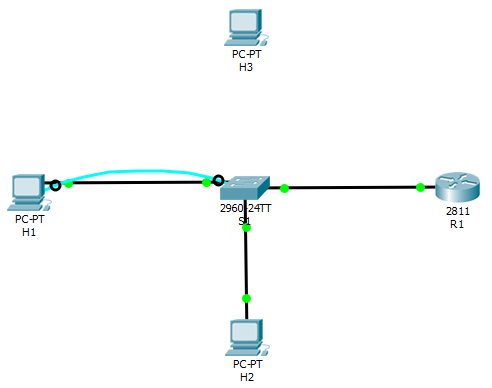
\includegraphics[width=0.6\linewidth]{Graphics/aufbau1.PNG}
  \caption{Versuchsaufbau - Teil 1}
  \label{fig:aufbau1}
\end{figure}

\begin{figure}[ht]
  \centering
     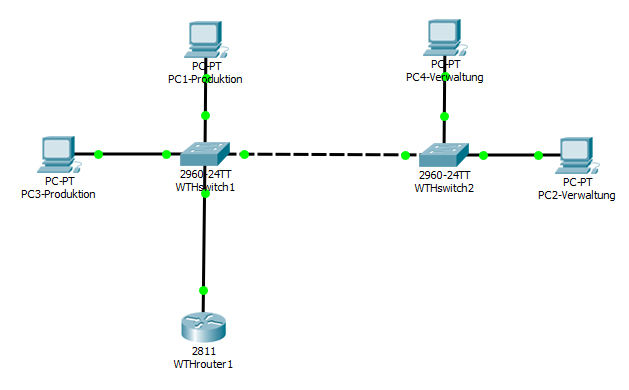
\includegraphics[width=0.6\linewidth]{Graphics/aufbau_2complete.PNG}
  \caption{Versuchsaufbau - Teil 2}
  \label{fig:aufbau2}
\end{figure}

% \subsection{Komponenten}
% 
% \begin{itemize}
%   	\item 3 Computer
%   	\item Cisco 2811 Router
%   	\begin{itemize}
%       	\item Verbindung zum Switch durch Straight-Through-Kabel
% 	\end{itemize}
%   	\item 1 Cisco 2960 Switch
%   		\begin{itemize}
%     	\item Verbindung zu Host 1 durch Straight-Through-Kabel und DB-9 zu
% 		RJ45 Adapterkabel
% 		\item Verbindung zu Host 2 durch Straight-Through-Kabel
%    		\end{itemize}
% \end{itemize}

\clearpage

\section{Versuchsdurchf�hrung}

Aus organisatorischen Gr�nden wurde dieser Laborversuch mittels
Cisco PacketTracer durchgef�hrt.

\subsection{Teil 1}\label{teil1}

\begin{table}[!htbp]
\centering
\small
	\begin{tabularx}{1.05\textwidth}{|X|X|X|X|X|X|X|}
	\hline
	\textbf{Device} & \textbf{Hostname} & \textbf{Interface} & \textbf{IP-Address} &
	\textbf{Subnet Mask} & \textbf{Default Gateway} & \textbf{Switch Port}\\
	\hline
	S1 	& Customer-Switch  & VLAN 1 & 192.168.1.5 & 255.255.255.0 & 192.168.1.1 &
	N/A \\
	\hline
	R1 & Customer-Router & Fa0/1 & 192.168.1.1 & 255.255.255.0 & N/A & Fa0/5 \\
	\hline
	H1 & H1 & NIC & 192.168.1.2 & 255.255.255.0 & 192.168.1.1 & Fa0/11 \\
	\hline
	H2 & H2 & NIC & 192.168.1.4	& 255.255.255.0 & 192.168.1.1 & fa0/18 \\
	\hline
	H3 & H3 & NIC & 192.168.1.6 & 255.255.255.0 & 192.168.1.1 & None \\
	\hline
	\end{tabularx}
\caption{Konfiguration f�r Teil 1}
\label{config1}
\end{table}

\underline{Weiteres Vorgehen:}
\begin{itemize}
  \item Initiale Switch-Konfiguration
  \item Hosts konfigurieren und mit Switch verbinden
  \item Router konfigurieren und mit Switch verbinden
  \item Switch Management VLAN IP-Adresse konfigurieren
  \item �berpr�fung der Netzwerk-Verbindungen
  \item Basic Port Security konfigurieren
  \item Port Duplex und Geschwindikeit konfigurieren
\end{itemize}

\subsection{Teil 2}\label{teil2}



\underline{Weiteres Vorgehen:}
\begin{itemize}
  \item Initiale Switch-Konfiguration
  \item VLAN-Konfiguration
  \item InterVLAN-Routing
\end{itemize}

\section{Versuchsziel}

